\chapter{Deployment}\label{ch:deployment}

\section{Data Stores}\label{sec:data-stores}

State in Anubis is somewhat fluid.
Data is parked either in the main Mariadb~\ref{subsec:mairadb} database, or
in the redis cache~\ref{subsec:caching}.

\subsection{Mariadb}\label{subsec:mariadb}

The main data store for Anubis is a \href{https://mariadb.org/}{MariaDB}
\href{https://mariadb.com/kb/en/galera-cluster/}{galera} deployment.
More specifically the
\href{https://github.com/bitnami/charts/tree/master/bitnami/mariadb-galera}{Bitnami mariadb-galera} chart is used.

The advantage of galera is that MariaDB is multi-leader.
Any node of the MariaDB cluster can be read or written to at any time.
In a multi leader database deployment there is a certain tolerance of downed nodes before
service is degraded.
Even if nodes begin to fail, the MariaDB pods that are available can still handle
read and write operations.

All persistent storage in Anubis is parked in MariaDB.
Things like student, course and assignment information are stored here.
Temporary values like autograde results are stored in redis~\ref{subsec:redis}.

\subsection{Redis}\label{subsec:redis}

\href{https://redis.io/}{Redis} in Anubis is where temporary values are stored.
It is assumed that redis is not persistent.
What this means is that the redis deployment should be able to be reset
at any time without critical data loss.
If and when values need to be persisted, MariaDB~\ref{subsec:mariadb} is the better option.

\subsection{Caching}\label{subsec:caching}

Caching in Anubis is handled by the
\href{https://flask-caching.readthedocs.io/en/latest/index.html}{flask-caching} library.
The return values for specific functions can be temporarily stored in Redis for some
period of time.

In the Anubis API there is a great deal of caching.
Almost all view functions that query for database values will cache the results in redis
for some period of time.

Many of the computationally intensive calculation results are cached.
Take the autograde results for example.
To calculate the best submission for a student, all the
calculated submission results for that student and assignment must be pulled
out of the database and examined.
Depending on the student and assignment, this calculation could involve
examining hundreds of submissions searching for the best.
The results for these autograde calculations are then stored in the cache.

For a 3 week window around each assignment deadline the autograde results
for the assignment are periodically calculated.
The purpose of this preprocessing is to ensure that the autograde results
for recent assignments are always available in the cache.
Without this small optimization, the autograde results page in the admin
panel would just about always require 15-30 seconds to load data.

Another example of heavy caching in Anubis would be the public usage visuals.
The visuals themselves are png images that are generated from matplotlib.
To generate the png we must periodically pull out all the submission
and cloud ide session information.
Pulling this data then generating the png can take upwards of 45 seconds to a minute.
45 seconds is obviously an unacceptable amount of time to wait for an image to load
in the browser.
Anubis handles this situation by telling the API to always load the cached png image
from the cache.
The image is then periodically re-generated in the Reaper Cronjob.

Without heavy caching on things like the autograde results and visual generation
the admin panel would be quite slow.

\subsection{RPC Queues}\label{subsec:rpc-queues}

Redis is also used as an RPC broker for the \href{https://python-rq.org}{python-rq}
library.
RPC job information can be sent to redis by the api.
Deployments of RPC workers can then pick up jobs for the queues that are assigned to them.

As stated before, Redis in Anubis is meant to be destroyable.
When Redis is destroyed, all the currently enqueued RPC jobs will be deleted along with it.
Often this is not the biggest deal in the world.
The reaper cron~\ref{sec:reaper} is very good at spotting inconsistencies from events like
Redis kicking over and fixing them.

\section{Logging}\label{sec:logging}

Logging in Anubis is handled by a few products in the \href{https://elastic.co}{elastic} ecosystem.

\subsection{Filebeat}\label{subsec:filebeat}

Filebeat is a log capturing tool that runs in the kube-system namespace.
It is configured to capture all container logs in the anubis kubernetes namespace.
The captures logs are then sent to elasticsearch for indexing.

The result of this setup is that we can just print out whatever logs we need to in
whatever pod/container in the anubis namespace, and they will be captured and indexed.

\subsection{Elasticsearch}\label{subsec:elasticsearch}

Anubis uses \href{https://www.elastic.co/elasticsearch/}{elasticsearch} as a search engine for logging, and event tracking.
The elastic ecosystem has other tools like \href{https://www.elastic.co/kibana/}{kibana} for visualizing data.
Other than the visualization features, elastic allows us to simply start throwing
data at it without defining any meaningful shape. 
This allows us to just log events and data into elastic to be retrieved, and visualized later.

Kibana is not packaged with Anubis anymore because it is not used often enough
to merit the memory resources that it requires.

\section{Kubernetes}\label{sec:kubernetes}

Anubis is heavily integrated with concepts of \href{https://kubernetes.io/}{Kubernetes} (also called k8s).
Features from this container orchestrator are used to make all of the fancy things
that Anubis can do possible.
Things like the Anubis Cloud IDEs~\ref{ch:cloud_ides} would simply not exist
without pod scheduling and resource scaling.

\subsection{Helm Chart}\label{subsec:helm-chart}

Helm is like a package manager for Kubernetes.
Kubernetes configuration is all in yaml files.
Helm enables an application to be packaged in template yaml files.
A \textit{values.yaml} file can then provided to fill in variables in the template yaml.
A helm package is called a chart.

Anubis is packaged as a helm chart.
By doing this, Anubis is an application that can be \textit{installed} to any k8s cluster
(with some minor configuration of course).

There are several options for how to deploy anubis that can be specified when running 
the deploy script at \textit{kube/deploy.sh}. 
Notable options are deploying in debug mode, setting the api replica count, or disabling rolling updates.
Options passed to the deploy script will be then passed to helm.

\begin{minted}{shell}
# Deploy in debug mode
./k8s/deploy.sh --set debug=true

# Set the initial number of replicas for the api service to 5
./k8s/deploy.sh --set api.replicas=5

# Disable rolling updates
./k8s/deploy.sh --set rollingUpdates=false
\end{minted}

\subsection{Longhorn}\label{subsec:longhorn}

The \href{https://kubernetes.io/docs/concepts/storage/storage-classes/}{Kubernetes StorageClass} 
that Anubis uses is \href{https://longhorn.io/}{Longhorn}.
It allows us to have \href{https://kubernetes.io/docs/concepts/storage/persistent-volumes/#access-modes}{ReadWriteMany}
volumes for things like the Cloud IDEs.

All important data is stored on 3x replicated Longhorn StorageVolumes.
Those volumes all have at least daily snapshots taken of them.
At any given time, we can reset any stateful service to a previous snapshot from the last seven days.

For the things that are very important we have daily snapshots, and extra replication.
Longhorn makes this as simple as checking some boxes.
You can see here our mariadb~\ref{subsec:mariadb} 0 replica with triple replication, 
with a 7 day snapshot.

\begin{figure}
    \centering
    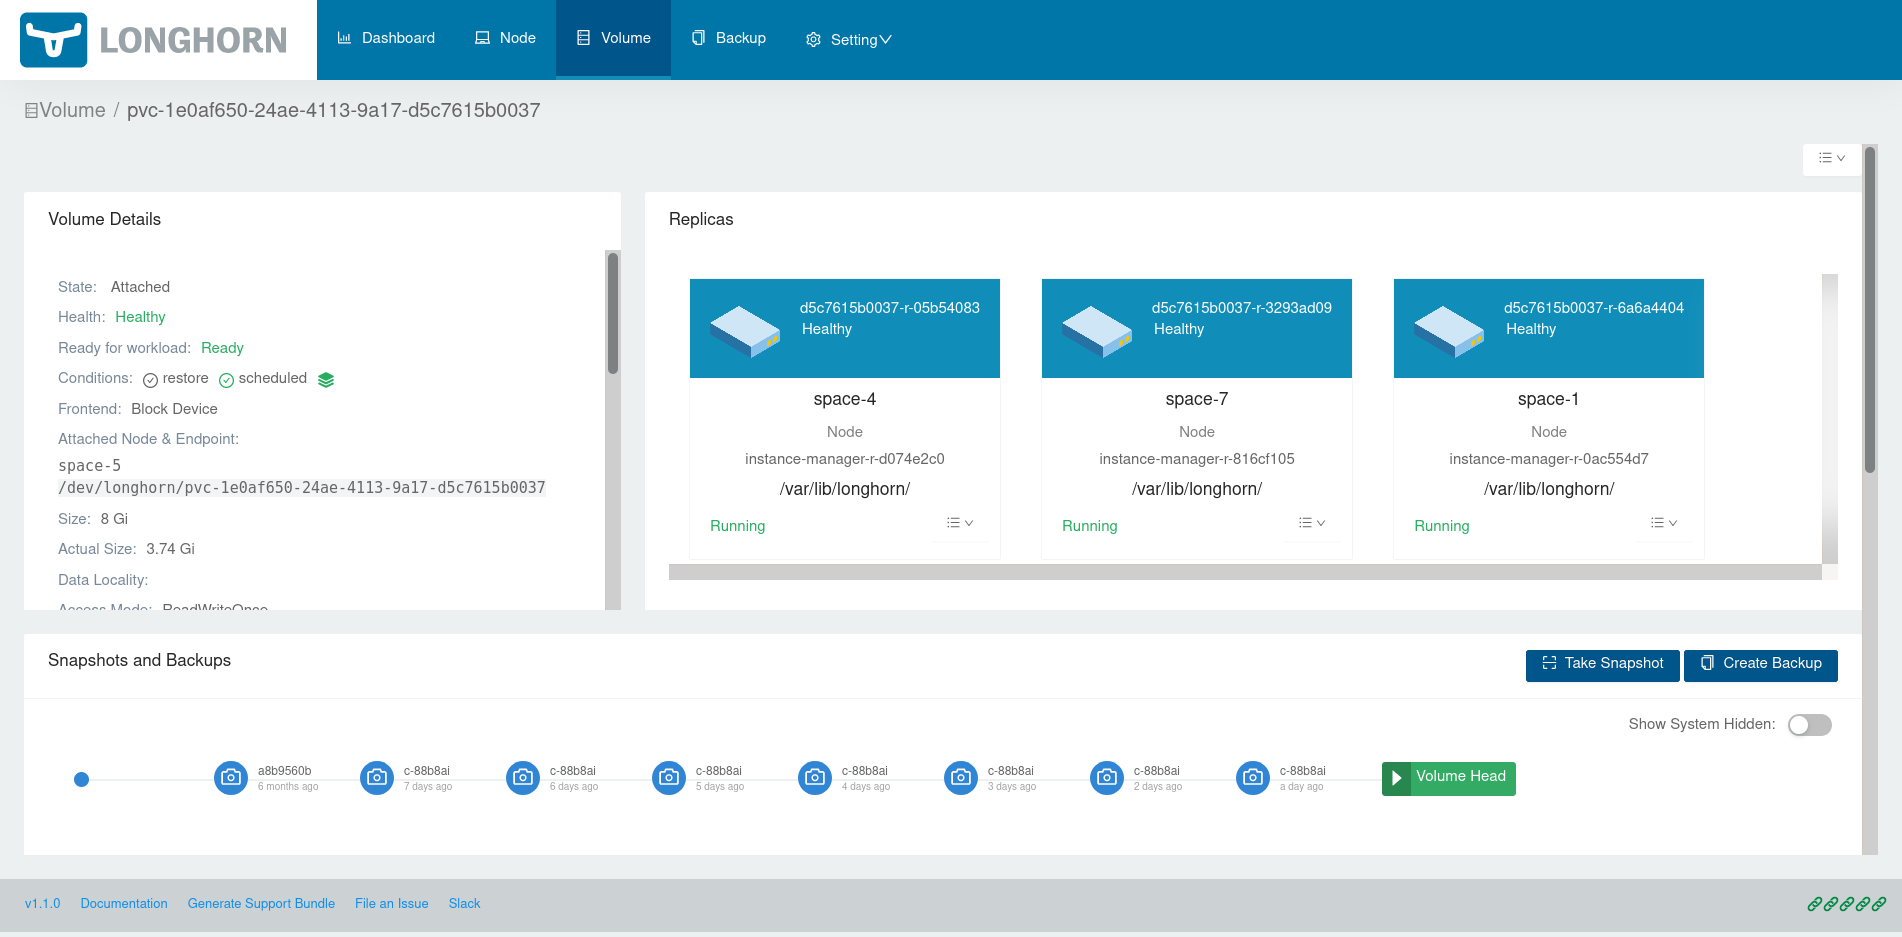
\includegraphics[width=0.5\textwidth]{figures/longhorn-mariadb}
\end{figure}

\subsection{Digital Ocean}\label{subsec:digital-ocean}

Anubis runs on a managed Kubernetes cluster in Digital Ocean.
Most hosting providers now have their own one click managed Kubernetes clusters.
The advantage of using a managed k8s cluster is that generally node autoscaling is
a feature that you can enable.

\subsubsection{Nodes}\label{subsubsec:digital-ocean-nodes}

The Anubis cluster on Digital Ocean are set to autoscale node pools.
Kubernetes keeps track of reserved resources (like cpu and memory) and will
report \textit{resource pressures} to digital ocean.
When that happens, more nodes will automatically be added to the cluster.

The autoscaling node pools is how autoscaling works in Anubis.
When a student creates a Cloud IDE, and the cluster does not have the cpu or 
memory resources, Digital Ocean will automatically add another node to handle the load.

\subsubsection{Networking}\label{subsubsec:digital-ocean-networking}

Anubis is accessed though a \href{https://docs.digitalocean.com/products/networking/load-balancers/}{Digital Ocean load balancer}.
The load balancer will be what has the external IP address for Anubis on the public internet.
Requests will then be balanced between all nodes to the traefik service.

\section{Github}\label{sec:github}

\subsection{Github Organizations}\label{subsec:github-orgs}

Each class has their own Github organization.
Repos generated through Github Classrooms~\ref{subsec:github-classrooms}
are then placed in the organization.

\subsection{Github Push Reporting}\label{subsec:github-push-reporting}

As explained in the assignment structure~\ref{sec:assignment-structure} section,
students get their own private repository for each assignment.
There are two ways that github reports submissions to Anubis.

The github organization's that use Anubis all have webhooks setup for push events.
This means that every time someone pushes to a repository in a github organization
that has Anubis assignment repos, github sends a webhook describing the push to
the Anubis api.
Unfortunately github has not always been the consistent about successful deliveries of
push event webhooks.
In earlier versions of Anubis, webhooks would often fail.
This would result in submissions basically getting lost.
The next option exists to solve this issue of lost submissions.

The second way that Anubis detects pushes to assignment repos is by the github API.
In the reaper job~\ref{sec:reaper} that runs every few minutes, a call is made to the
github api to list all recent commits to repositories in github organizations that
Anubis is responsible for.
If a commit is seen in this api response that was not reported by a webhook,
a submission record is created and a pipeline enqueued.

\subsection{Github Classrooms}\label{subsec:github-classrooms}

Student's get their own github repositories for each assignment in Anubis.
The way that these repositories are created for students is through github classrooms.
Classrooms is an integration into each classes github organization.
Assignments in classrooms can then be created by specifying a template repository.
Students then use the link that classroom gives to generate their own repositories~\ref{fig:github-classroom-1}.

\begin{figure}
    \centering
    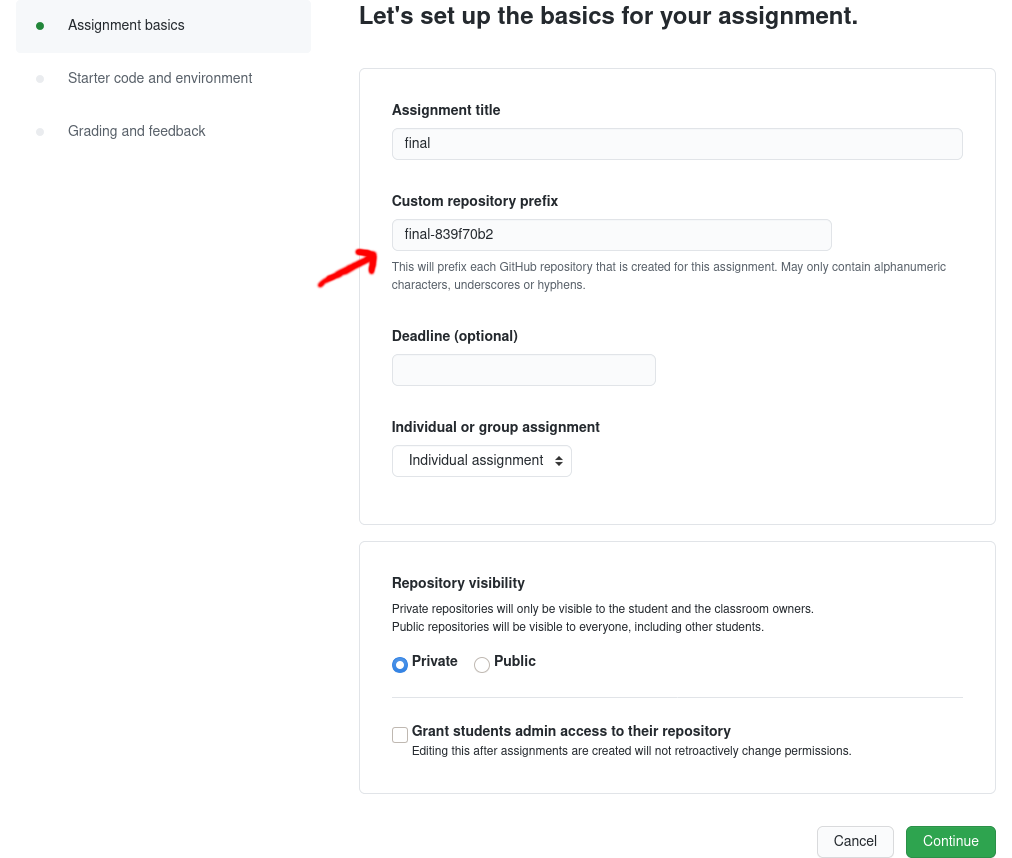
\includegraphics[width=0.5\textwidth]{figures/github-classroom-1}
    \caption{Assignment Repo Creation Link\label{fig:github-classroom-1}}
\end{figure}

Anubis has a problem to contend with here.
When Anubis picks up submissions in repos, it needs to be able
to tell which assignments on Anubis get matches to which repos.
The solution Anubis uses to solve this is a short unique hash identifier 
for each assignment.
When creating the assignment on github classroom, a prefix for the title in the repo
can be specified~\ref{fig:github-classroom-2}.
The unique hash identifier to be used here is created in the meta.yaml file in the assignment
tests, and available in the assignment management page on the web admin panel.

\begin{figure}[ht]
    \centering
    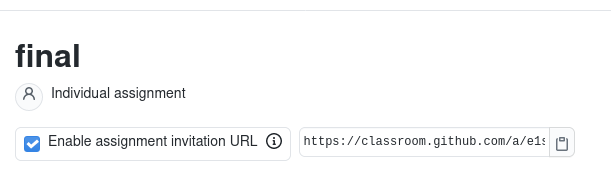
\includegraphics[width=0.5\textwidth]{figures/github-classroom-2}
    \caption{Github Classroom Repo Prefix\label{fig:github-classroom-2}}
\end{figure}
